%******************************************************************************%
%                                                                              %
%                  html_css.en.tex for LaTeX                             %
%                  Created on : Tue Mar 10 13:27:28 2015                       %
%                  Made by : Dax Wann                                          %
%                                                                              %
%******************************************************************************%

\documentclass{42-en}

%******************************************************************************%
%                                                                              %
%                                    Header                                    %
%                                                                              %
%******************************************************************************%
\begin{document}



                           \title{Responsive Web Design}
                          \subtitle{FreeCodeCamp edition}
                       \member{Dax Wann}{daxwann@gmail.com}
                        \member{42 Staff}{pedago@42.fr}

\summary {
  An introduction to designing responsive websites with HTML and CSS.
}

\maketitle

\tableofcontents


%******************************************************************************%
%                                                                              %
%                                  Foreword                                    %
%                                                                              %
%******************************************************************************%
\chapter{Foreword}

    \begin{figure}[H]
        \begin{center}
            
\includegraphics[width=12cm]{thor.jpg}
        \end{center}
    \end{figure}
    [Thor is trying to access on the Quinjet’s computer]\\
Quinjet Computer: Welcome. Voice activation required.\\
Thor: Thor.\\
Quinjet Computer: Access denied.\\
Thor: Thor, son of Odin.\\
Quinjet Computer: Access denied.\\
Thor: God of Thunder.\\
Quinjet Computer: Access denied.\\
Thor: Strongest Avenger.\\
Quinjet Computer: Access denied.\\
Thor: Strongest Avenger.\\
Quinjet Computer: Access denied.\\
Thor: Damn you, Stark. Point Break.\\
Quinjet Computer: Welcome, Point Break.\\
\\
- \textit{Thor: Ragnarok}
    
%******************************************************************************%
%                                                                              %
%                                 Introduction                                 %
%                                                                              %
%******************************************************************************%
\chapter{Introduction}

It's time to learn how to build a website for the world to see! We will first focus on making a static website. A simple static website consists of HTML (HyperText Markup Language) and CSS (Cascading Style Sheet). HTML is used to create the structure of the website, such as text, images, and other media. CSS is used to style those structures, such as changing the color of the text, the size of the images, and layout of the page.\\
    
\textbf{HTML}: structure and content of the website\par
\textbf{CSS}: style and layout of the website\\

With the skills of using HTML and CSS, you will be able to design websites that's appealing, accessible, and responsive to the user's devices.



%******************************************************************************%
%                                                                              %
%                                  Goals                                       %
%                                                                              %
%******************************************************************************%
\chapter{Goals}

Using FreeCodeCamp online curriculum, we will learn:
\begin{itemize}
    \item basic HTML
    \item basic CSS
    \item applied visual design
    \item Responsive web design principles
    \item CSS Flexbox
    \item CSS Grid
\end{itemize}

For our culminating project, we will apply what we learned to create a responsive tribute website of a personal hero. We will push our project onto a Github repository and deploy our website with Github Pages to showcase.



%******************************************************************************%
%                                                                              %
%                             General instructions                             %
%                                                                              %
%******************************************************************************%
\chapter{General instructions}

\begin{enumerate}
    \item Create an account on \url{https://www.freecodecamp.org/} using your personal email
    \item Click on "Curriculum" in the top right corner
    \item Finish the mandatory sections listed on the next page
    \item Create \textbf{responsive} website of a personal hero using HTML5 and CSS3
    \item Create a free account on \url{https://github.com/} using your personal email
    \item Push project onto a new Github repository
    \item Deploy website on Github Pages
\end{enumerate}
   
    



%******************************************************************************%
%                                                                              %
%                             Mandatory part                                   %
%                                                                              %
%******************************************************************************%
\chapter{Mandatory part}

Finish all exercises in these following sections on FreeCodeCamp Responsive Web Design Certificate:
\begin{itemize}
    \item Basic HTML and HTML5
    \item Basic CSS
    \item Applied Visual Design
    \item Responsive Web Design Principles
    \item CSS Flexbox
    \item CSS Grid
\end{itemize}
\vspace{0.2in}

Create a responsive website about a personal hero using HTML5, CSS3, CSS Flexbox and/or Grid.\par
\vspace{0.2in}
Push your website project repository onto your Github. Deploy your website on github.io.
    


%******************************************************************************%
%                                                                              %
%                             Exercises of a Piscine                           %
%                                                                              %
%******************************************************************************%

\chapter{Exercise 00: FreeCodeCamp}

\extitle{Sign up on \href{FreeCodeCamp}{FreeCodeCamp}}
\exnumber{\exercicenumber}
\exscore{2}
\exfiles{n/a}
\exauthorize{All}

\makeheaderfiles

Go to \url{https://www.freecodecamp.org/} and create an account using a personal email. In "Curriculum", go to Responsive Web Design Certificate section.

%******************************************************************************%
%                                                                              %
%                             Exercises of a Piscine                           %
%                                                                              %
%******************************************************************************%

\chapter{Exercise 01: Basic HTML and HTML5}

\extitle{Basic HTML and HTML5 on FreeCodeCamp}
\exnumber{\exercicenumber}
\exscore{2}
\exfiles{All exercises completed in section on FreeCodeCamp}
\exauthorize{All}

\makeheaderfiles

HTML is used to create a structure for contents in the website. Usually websites will have a header and a body. A website can also include text, images, videos, and other media.

%******************************************************************************%
%                                                                              %
%                             Exercises of a Piscine                           %
%                                                                              %
%******************************************************************************%

\chapter{Exercise 02: Basic CSS}

\extitle{Basic CSS on FreeCodeCamp}
\exnumber{\exercicenumber}
\exscore{2}
\exfiles{All exercises completed in section on FreeCodeCamp}
\exauthorize{All}

\makeheaderfiles

CSS is used to style the structures created in HTML. For example, we use CSS to change fonts, text sizes, background color, image sizes, etc. We also use CSS to create overall layout of the website. You will learn more layout functionalities later with CSS Flexbox and CSS Grid.

%******************************************************************************%
%                                                                              %
%                             Exercises of a Piscine                           %
%                                                                              %
%******************************************************************************%

\chapter{Exercise 03: Applied Visual Design}

\extitle{Applied Visual Design on FreeCodeCamp}
\exnumber{\exercicenumber}
\exscore{2}
\exfiles{All exercises completed in section on FreeCodeCamp}
\exauthorize{All}

\makeheaderfiles

We will now learn more about designing a website using CSS. A website would be frustrating for the users if its design was not well thought out. For example, we should make the text big enough for users to read easily. We should highlight the important content. We should use colors and images to support our main content.

%******************************************************************************%
%                                                                              %
%                             Exercises of a Piscine                           %
%                                                                              %
%******************************************************************************%

\chapter{Exercise 04: Responsive Web Design Principles}

\extitle{Responsive Web Design Principles on FreeCodeCamp}
\exnumber{\exercicenumber}
\exscore{2}
\exfiles{All exercises completed in section on FreeCodeCamp}
\exauthorize{All}

\makeheaderfiles

Since users can view our website with different devices in various sizes, such as on a laptop, a gaming monitor, a mobile phone, or an iPad, we need to make our website adapt to the screen size. We use responsive web design to create different styles and layouts for different device sizes.

%******************************************************************************%
%                                                                              %
%                             Exercises of a Piscine                           %
%                                                                              %
%******************************************************************************%

\chapter{Exercise 05: CSS Flexbox}

\extitle{CSS Flexbox on FreeCodeCamp}
\exnumber{\exercicenumber}
\exscore{2}
\exfiles{All exercises completed in section on FreeCodeCamp}
\exauthorize{All}

\makeheaderfiles

CSS Flexbox is a new responsive layout feature that will help arrange elements within a parent container.\par
\vspace{.2in}
Learn more about CSS Flexbox here: \par
\url{https://css-tricks.com/snippets/css/a-guide-to-flexbox/}

%******************************************************************************%
%                                                                              %
%                             Exercises of a Piscine                           %
%                                                                              %
%******************************************************************************%

\chapter{Exercise 06: CSS Grid}

\extitle{CSS Grid on FreeCodeCamp}
\exnumber{\exercicenumber}
\exscore{2}
\exfiles{All exercises completed in section on FreeCodeCamp}
\exauthorize{All}

\makeheaderfiles

Similar to Flexbox, CSS Grid is another responsive layout feature that will help arrange elements within a parent container.\par
\vspace{.2in}
Learn more about CSS Grid here: \par
\url{https://css-tricks.com/snippets/css/complete-guide-grid/}

%******************************************************************************%
%                                                                              %
%                             Exercises of a Piscine                           %
%                                                                              %
%******************************************************************************%

\chapter{Exercise 07: Responsive Web Design Project}

\extitle{Responsive Web Design Project}
\exnumber{\exercicenumber}
\exscore{2}
\exfiles{Your project folder should include index.html, style.css, and image files in "assets/" subdirectory}
\exauthorize{All}

\makeheaderfiles

Create a tribute website of a person you are inspired by, like an artist, athelete, author, actor, etc. \par
\vspace{.1in}
The website should:
\begin{itemize}
    \item be responsive to mobile, iPad, and desktop screens
    \item have header, main content, a sidebar, and a footer in desktop view
    \item should have two or more containers occupying the row direction in desktop view
    \item should have only one container occupying the row direction in mobile view
    \item include mostly images with captions, one or two lists, few texts, two or more background colors, and one or more custom fonts
    \item should use CSS Flexbox and/or CSS Grid in the responsive design
\end{itemize}
\vspace{.5in}
Use the wireframes below for inspiration
\begin{figure}[H]
    \begin{center}
        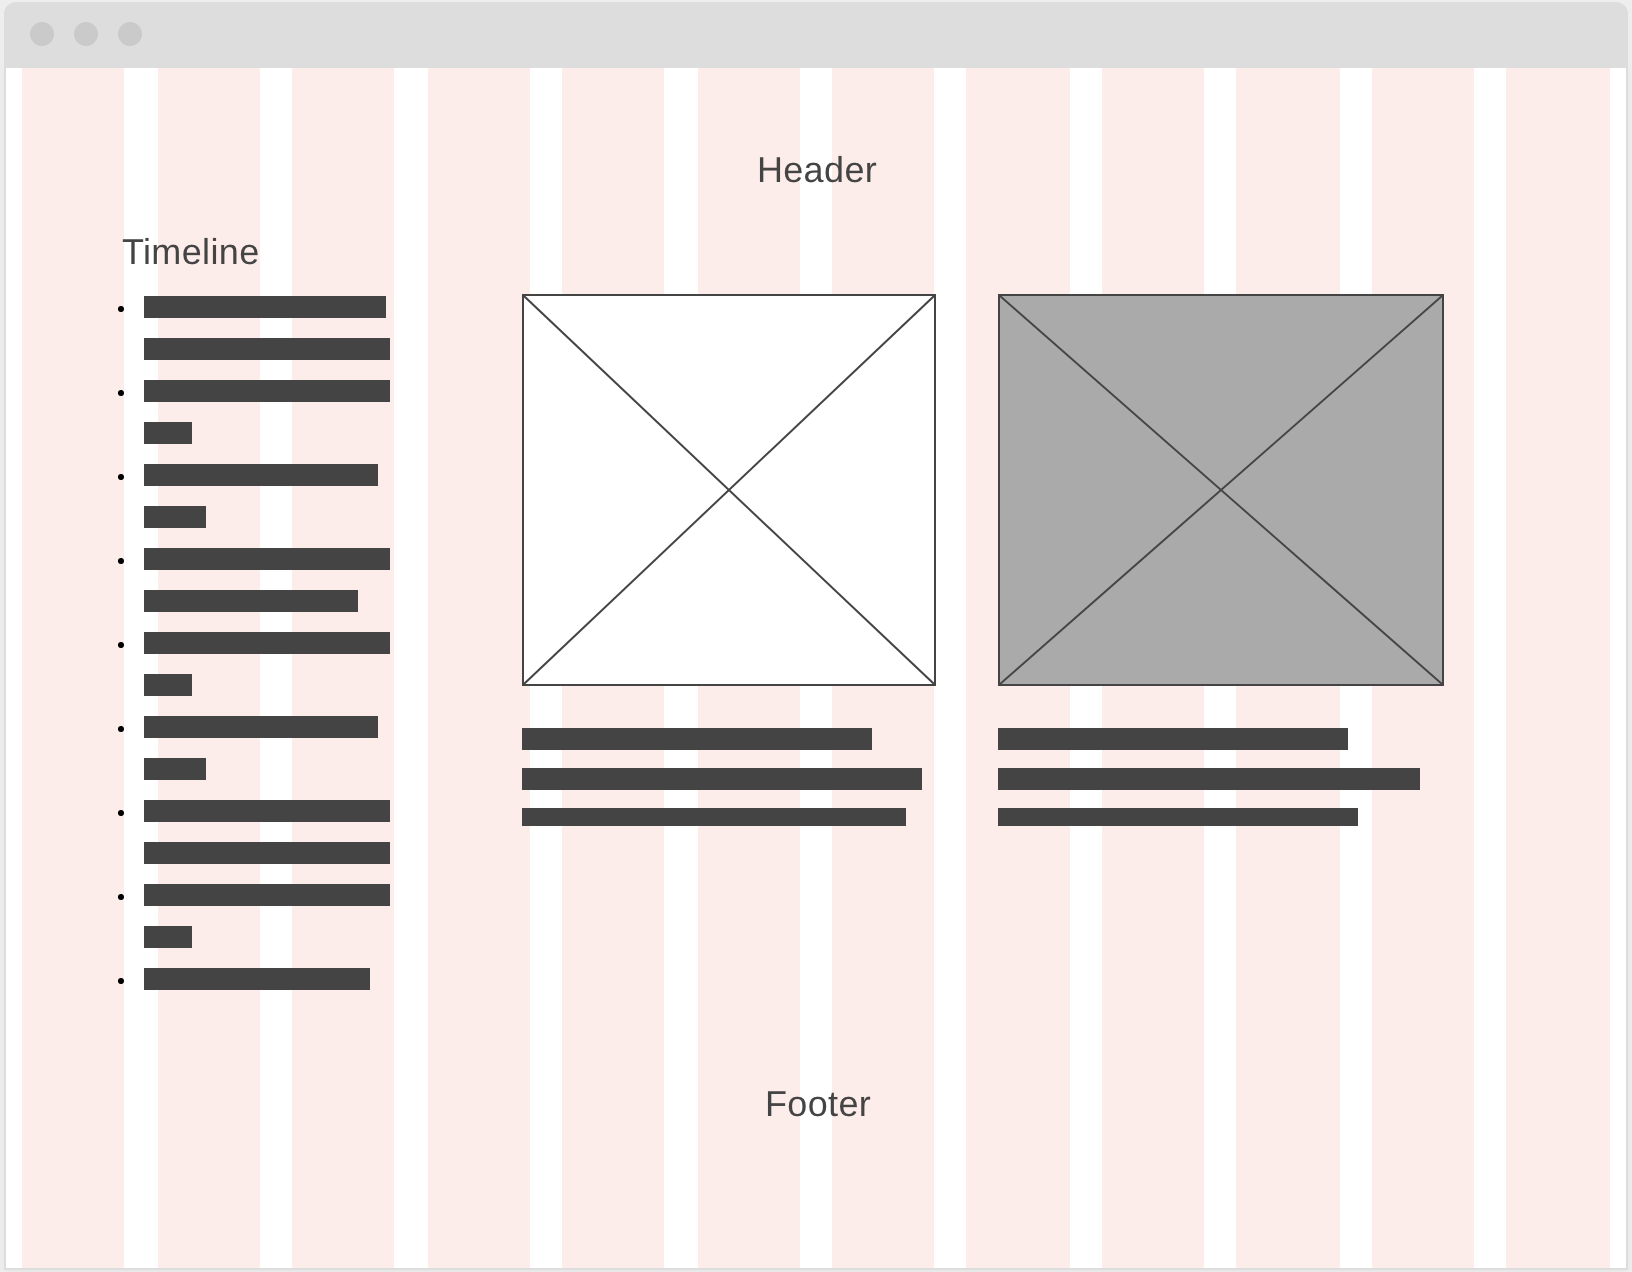
\includegraphics[width=12cm]{wireframe_desktop.png}\\
        desktop view
    \end{center}
\end{figure}
    
\begin{figure}[H]
        \begin{center}
            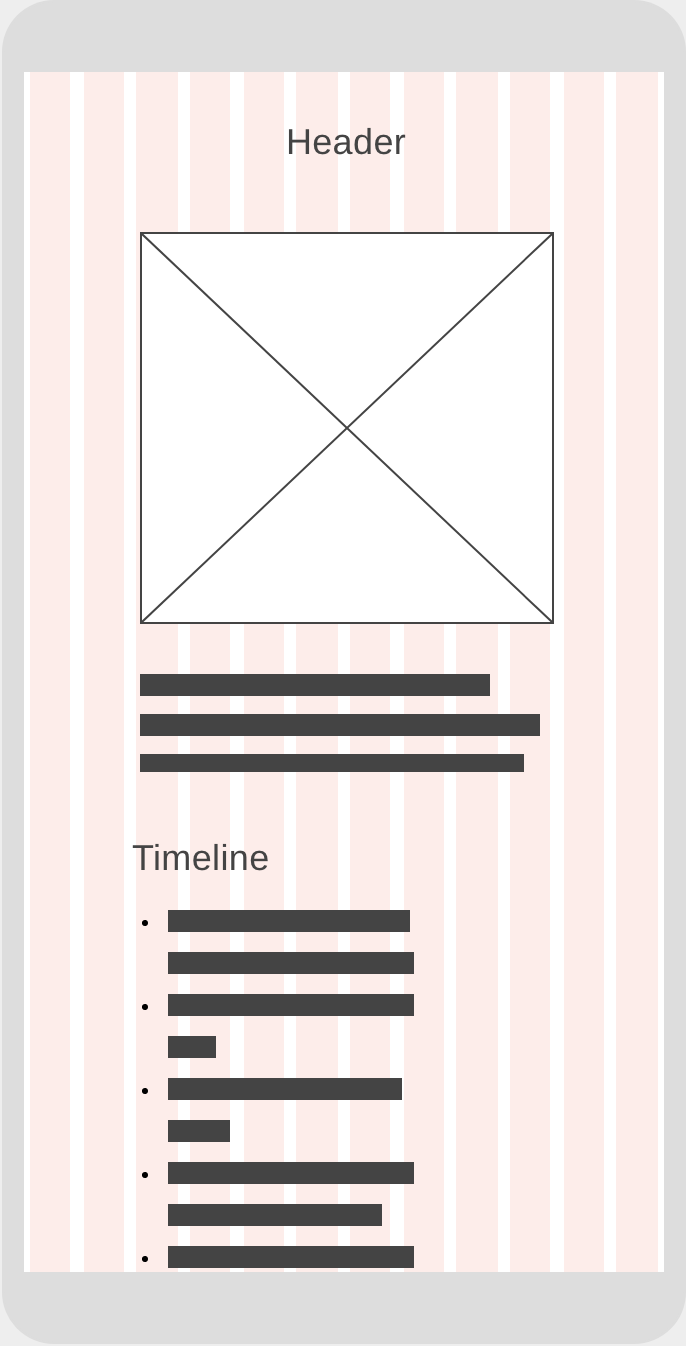
\includegraphics[width=4cm]{wireframe_mobile.png}\\
            mobile view
        \end{center}
    \end{figure}
\textbf{Suggestions}
\begin{enumerate}
    \item Create a project folder along with files \texttt{index.html} and \texttt{style.css}. Create a subfolder named \texttt{assets/} for images
    \item Use Visual Studio Code IDE to open the folder and start writing the HTML and CSS
    \item Apply what you learned in FreeCodeCamp to create the structure of the website and style it
    \item Use Chrome browser to test your website. You can access your website by opening the html file with Chrome or typing in its file path in the browser. If you are stuck, google first.
    \item Be sure to make the website responsive. Use \href{https://developers.google.com/web/tools/chrome-devtools/device-mode}{Chrome Developer Tools} to help you view your website on different devices.
\end{enumerate}

%******************************************************************************%
%                                                                              %
%                             Exercises of a Piscine                           %
%                                                                              %
%******************************************************************************%

\chapter{Exercise 08: Github}

\extitle{Create github account}
\exnumber{\exercicenumber}
\exscore{2}
\exfiles{Your Github repository should include \texttt{index.html}, \texttt{style.css}, and image files in \texttt{assets/} subdirectory}
\exauthorize{All}

\makeheaderfiles

\begin{enumerate}
    \item Go to \url{https://github.com/} and create a free account using your personal email if you don't already have one
    \item Create a new public repository named \texttt{H2S\_responsive\_tribute\_page}
    \item Follow \href{https://help.github.com/en/articles/adding-a-remote}{instructions} on connecting your tribute website project to the new Github repository
    \item Push your project onto the Github repository
    \item Go to your Github repository settings, under "Github Pages", publish your project as a website. Follow the URL formatted as
    \begin{center}
        \texttt{<username>.github.io/H2S\_responsive\_tribute\_page} \\
    \end{center}
    to view website.
    \item Create a \texttt{README.md} in the root directory of your project folder and copy the website URL into it. Follow this \href{https://help.github.com/en/articles/basic-writing-and-formatting-syntax#headings}{guide}.
\end{enumerate}

%******************************************************************************%
%                                                                              %
%                           Turn-in and peer-evaluation                        %
%                                                                              %
%******************************************************************************%
\chapter{Turn-in and peer-evaluation}

    Check that all exercises in the previously listed FreeCodeCamp sections have been completed.\\
    
    Check website is published on Github Pages.\\

    Turn your source code in using your \texttt{42 Git repository}. Only work present on your repository will be graded in defense.

%******************************************************************************%
\end{document}
